
\chapter{Prestatie verwachtingen}
\label{Prestatie_verwachtingen}
\textit{In dit hoofdstuk worden de prestaties verwachtingen toegelicht aan de hand van de in \cref{cha:opdrachtanalyse} opgestelde prestatie criteria (\cref{se:PC}) en functionele eisen (\cref{se:PVE}). In \cref{se:presentatie_ontwerp} wordt het ontwikkelde concept gepresenteerd, hier wordt een korte omschrijving van het ontwerp gegeven samen met een afbeelding. In \cref{se:prestatie_en_eigenschappen} worden de verwachte prestaties verteld met eventuele berekeningen om dezen te ondersteunen, ook worden hier de specifieke eigenschappen van het ontwerp toegelicht. In \cref{se:veiligheidsanalyse_prestatieverwachting} wordt een veiligheid-overzicht van het ontwerp gepresenteerd.}

\section{Presentatie van het ontwerp}
\label{se:presentatie_ontwerp}

De Driepoter is een ontwerp dat in staat is om over obstakels heen te stappen door middel van zijn inklapbare poten. Zoals te zien is in \cref{fig:De_driepoter_Prestatie_analyse} is de Driepoter in staat om de schaarliften die hij aan de onderkant van het chassis heeft in te klappen en uit te klappen. De Driepoter kan het pakket ontvangen door middel van een rol-baar plateau, dit zorgt ervoor dat de Drieklapper een verstelbaar zwaarte punt heeft wat handig is voor het nemen van een talud. Eenmaal wanneer de Driepoter een bocht moet maken kan hij zien voorste wielen draaien en net als een auto een bocht maken.\\

\vspace{\baselineskip}
\begin{figure}[H]
    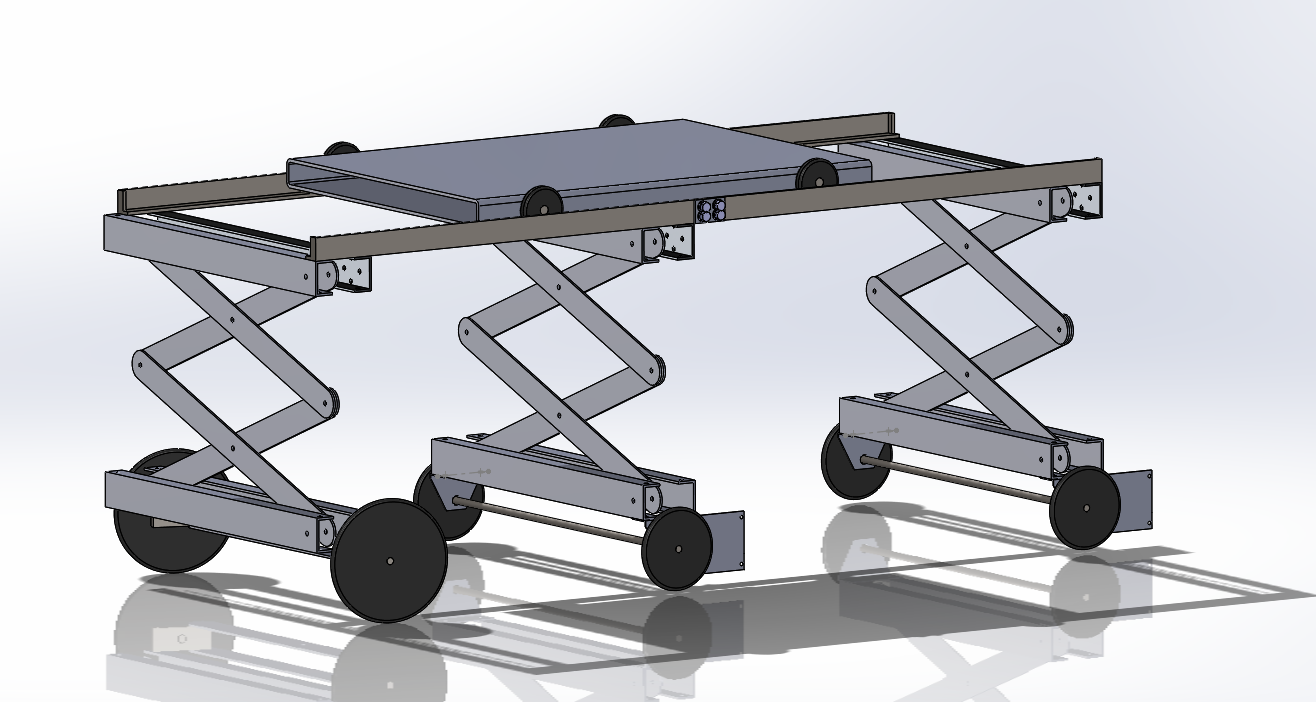
\includegraphics[width = 120mm]{04_gekozenconcept/eindconcept.png}
    \caption{de Driepoter}
    \label{fig:De_driepoter_Prestatie_analyse}
\end{figure}


\section{Verwachte eigenschappen en prestaties}
\label{se:prestatie_en_eigenschappen}
Hier worden de prestaties en de eigenschappen van de Driepoter besproken en onderbouwt door middel van berekeningen en bronnen. De mogelijke prestaties zijn aan de hand van de prestatie criteria en het programma van eisen in \cref{cha:opdrachtanalyse} opgesteld.

\subsection{Het gewicht van het pakket hondje}
Het is van belang voor verdere berekeningen en voor de prestatie van het pakkethondje om de totale massa van het ontwerp te bepalen.\\
Uit het solidworks model is gehaald dat de massa van het ontwerp x kg is, dit is echter maar een benadering van de werkelijkheid. Bij deze massa komen nog de massa 's van de wielen, de motoren en het te vervoeren pakket.\\

\subsection{De snelheid van het nemen van een talud}

\subsection{De snelheid van het nemen van de hindernisbaan}

\subsection{De stabiliteit tijdens het rijden}

\subsection{De stabiliteit tijdens het nemen van een talud}

\subsection{De benodigde hoeveelheid energie}

\subsection{Het pakketje moet voldoen aan de CE-norm}

\section{veiligheidsanalyse}
\label{se:veiligheidsanalyse_prestatieverwachting}

